
\documentclass[journal]{IEEEtran}
%\usepackage{lineno}
%\linenumbers
%\usepackage{cite}
\usepackage{comment}
\ifCLASSINFOpdf
  \usepackage[pdftex]{graphicx}
  \graphicspath{pics/}
  \DeclareGraphicsExtensions{.pdf,.jpeg,.png,.jpg}
\else

\fi
\usepackage{amsmath}
\usepackage{siunitx}
\usepackage{comment}
\usepackage[caption=false]{subfig}
\usepackage[super]{nth}
\hyphenation{}


\begin{document}
\title{22051 - Assignment number 1}
\author{\underline{Group 3}\\ s194048 Erik Rame (\_ hrs) \\ s194051 Jakob Bernhardt (\_ hrs) \\ s194006 Steffan Kunoy (\_ hrs) \\ s186083 Tjark Petersen (\_ hrs)}
%\markboth{Project description}%
%{}


% make the title area
\maketitle

%\IEEEpeerreviewmaketitle

\section{Summary and objectives}
The goal with these reports is to provide a situation where specific tasks need to be solved as a team and where results are documented in a professional and concise way. In addition, the contents of the hands-on will provide you with an idea of where you stand in the course relative to the learning objectives. While it might be hard in the beginning, documentation of results will play an increasing role in your career. Please follow below guidelines when preparing your report.

\subsection{Example text} 
The convolution operation plays an important role in signal processing. Knowing the impulse response of a linear, time-invariant system, the system output can be computed by convolution of an arbitrary input signal with the systems impulse resposne. The convolution theorem translates this operationn to the frequncy domain.
The first part of the report describes the filtering of a delicious chocolate cake through a infinite impulse response (IIR) filter, resulting in another declicious vanilla cake. The second part describes a running beer filter as a prototype for finite impulse response (FIR) filters. The characterization of the filter is described, along with the results of some arbitrary test signals.
The results show that you can also have fun at later stages of your academic career, and that it is actually tough to condense the information to its essentials when you only have 4 pages to fill including pictures.

\section{Methods}
Describe your methods here. Describe how you tackle the problem and why you think it is a good idea to do it exactly this way. Avoid lengthy repetition of the content of the book and restrict yourself to the most essentual information. Provide all the information required to reproduce your results one to one.

The optimal number of bicycles to have is given by eq. \ref{eq:bikes}
\begin{equation}\label{eq:bikes}
 N_b = n + 1 \qquad \mbox{constrained by:} \ \ N_b < s
\end{equation}

where $N_b$ refers to the optimal number of bicycles, $n$ to the number of bicycles you have at the moment, and $s$ the number of bicycles where your spouse will kick you out.


\subsection{Figures}
Prepare your figures such that they fit in width within one column, that the lines are visible and that all fonts are readable. As a guideline, the font size in the figures should be at least the size of the running text. Reduce the number of figures to a minimum. If you have a lot of information, provide panels and label each panel with a capital letter in the top left corner (i.e., A, B, C, ...). Refer to all figures in the running text.  

\subsection{Figure captions}
Please provide figure captions where you describe the main contents of the corresponding figure. This might look as in figure \ref{fig:eyes}:
\begin{figure}
 \includegraphics[width=\columnwidth]{eyes}
 \caption{These are eyes of some insect species. There are two of them, located on the left and on the right hand side. They look weird - and they will observe you if you do not follow the rules.}
 \label{fig:eyes}
\end{figure}


\newpage
\section{Simple filters with poles and zeros}
The objective of this exercise was to gain experience working with the \textit{z}-transform by manipulating the poles and zeros of filters and transfer functions. In particular, the tasks highlighted how the placement of poles and zeros on the unit circle dictated the characteristic frequency response of for example a running-sum or a high-pass filter. Further, we tried passing different types of signals through the filters to study the effect they had on them. 

\subsection{The z-transform}
Generally, the \textit{z}-transform of a discrete-time signal $x(n)$ into the complex \textit{z}-plane is given by the \textit{bilateral} forward transform: 
\begin{equation}
\label{eqn:z_transform}
    X(z) = \sum_{n=-\infty}^{\infty} x(n) \cdot z^{-n}
\end{equation}
However, since our signals are assumed to be causal, the \textit{unilateral} transform starting at $n=0$ is used. For instance, the \textit{z}-transform of a \nth{3} order running sum filter $h(n)$, which is simply a summation of 4 terms: 
\begin{equation}
\label{eqn:third_order_rs}
    H(z) = \sum_{n=0}^{\infty} h(n) \cdot z^{-n} = z^{0} + z^{-1} + z^{-2} + z^{-3} 
\end{equation}
As the \textit{z}-transform can be seen as a generalized case of the Fourier transform, the result can easily be mapped to the frequency domain using $z \rightarrow e^{j \omega}$.

\subsection{Poles and zeros}
Using algebraic manipulation, we can express the \textit{z}-transform of the \nth{3} order running sum filter in (\ref{eqn:third_order_rs}) as a ratio of polynomials: 
\begin{equation}
\label{eqn:third_order_rs_tf}
    H(z) = \frac{z^3+z^2+z^1+1}{z^3}
\end{equation}
The roots of the denominator and numerator polynomials, known as poles and zeros respectively, dictate the frequency response of an LTI-system with $H(z)$ as its transfer function. Thus, the third order running sum filter is seen to have a triple pole at $z=0$ and zeros at $z=-1$ and $z=\pm i$, as illustrated in the \textit{z}-plane plot in Figure \ref{fig:zplane_a}. Poles cause the transfer function value to go to infinity, while zeros cause it to go to zero. As a result, the frequency response of the filter, shown in Figure \ref{fig:freq_resp1_a}, is heavily attenuated at the normalized frequencies $\frac{\pi}{2}, \pi \text{ and } \frac{3 \pi}{2}$, corresponding to the arguments of each of the three zeros. Likewise, the frequency response of the \nth{5} order running sum filter in Figure \ref{fig:freq_resp1_b} is also affected by its pole-zero locations shown in Figure \ref{fig:zplane_b}. 

\subsection{Filtering} 
As seen in the previous section, we can control the frequency response of an LTI-system simply by placing its poles and zeros at appropriate locations on the \textit{z}-plane. Placing a single real zero at some distance $0<r<1$ from the origin and no poles creates a \textbf{low-pass} filter, while placing a single pole at the same distance without any zeros yields a \textbf{high-pass} filter. Placing an equal number of poles and zeros at the exact same locations meanwhile produces an \textbf{all-pass} filter. \\
Passing a signal through these filters requires convolution in the time domain, or simply multiplication in the \textit{z}-domain. Figure \_ shows the result of filtering a sinusoid with a low-pass, high-pass and all-pass filter. From this time-domain plot we can see that the low-pass filter attenuates the signal amplitude by a factor of $0.5$ while the high-pass filter amplifies it by a factor of 2. As expected, the all-pass filter has no effect on the signal amplitude. 

\subsection{Audio processing}
The synthesized filters can also be used on more complex signals, such as a sound signal. An example is shown in Figure \_, where a 5 ms sound clip has been passed through all filter types. 

\subsection{Plots}
\begin{figure}[h]
    \centering
    \captionsetup[subfloat]{farskip=0pt,captionskip=0pt}
    \subfloat[\nth{3} order running sum]{
        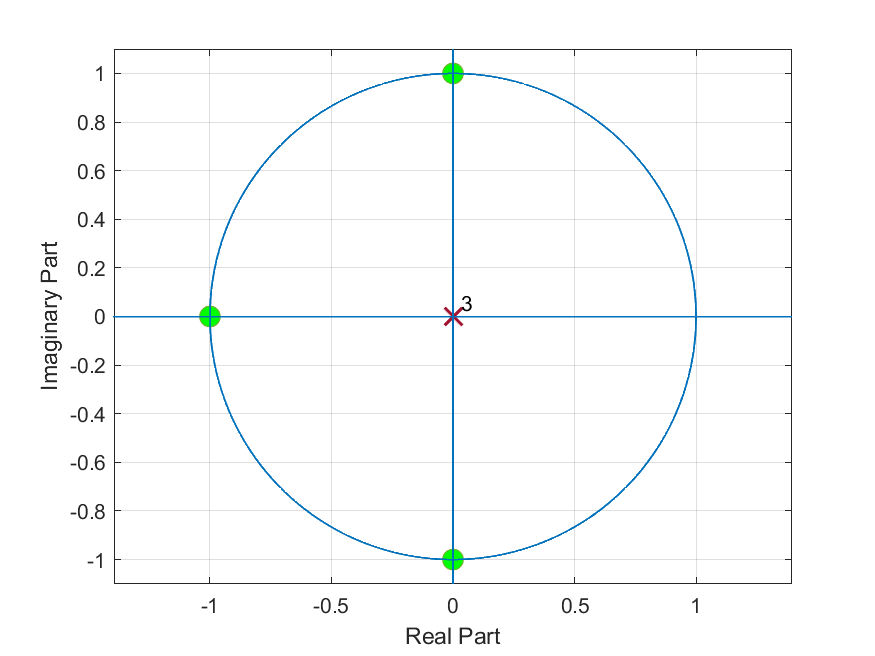
\includegraphics[width=0.5\columnwidth]{assignment_01/plots/3rd_order_running_sum_z_plane.png}
        \label{fig:zplane_a}
    }
    \subfloat[\nth{5} order running sum]{
        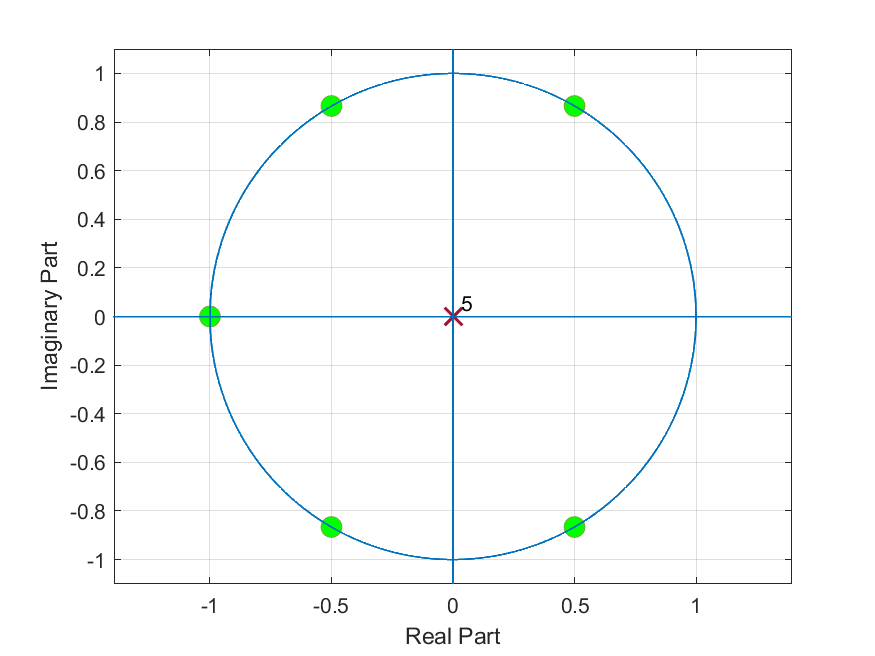
\includegraphics[width=0.5\columnwidth]{assignment_01/plots/5th_order_running_sum_z_plane.png}
        \label{fig:zplane_b}
    }
    \caption{Placement of poles and zeros of two running sum filters on the complex \textit{z}-plane.}
    \label{fig:zplane}
\end{figure}
\begin{figure}[h]
    \centering
    \captionsetup[subfloat]{farskip=0pt,captionskip=0pt}
    \subfloat[\nth{3} order running sum]{
        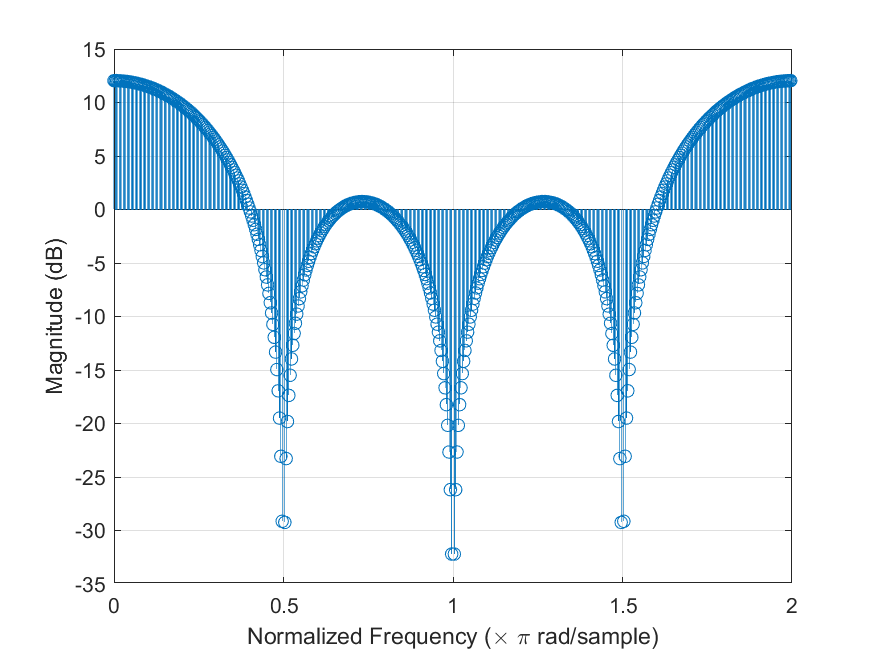
\includegraphics[width=0.5\columnwidth]{assignment_01/plots/3rd_order_running_sum_freq_resp.png}
        \label{fig:freq_resp1_a}
    }
    \subfloat[\nth{5} order running sum]{
        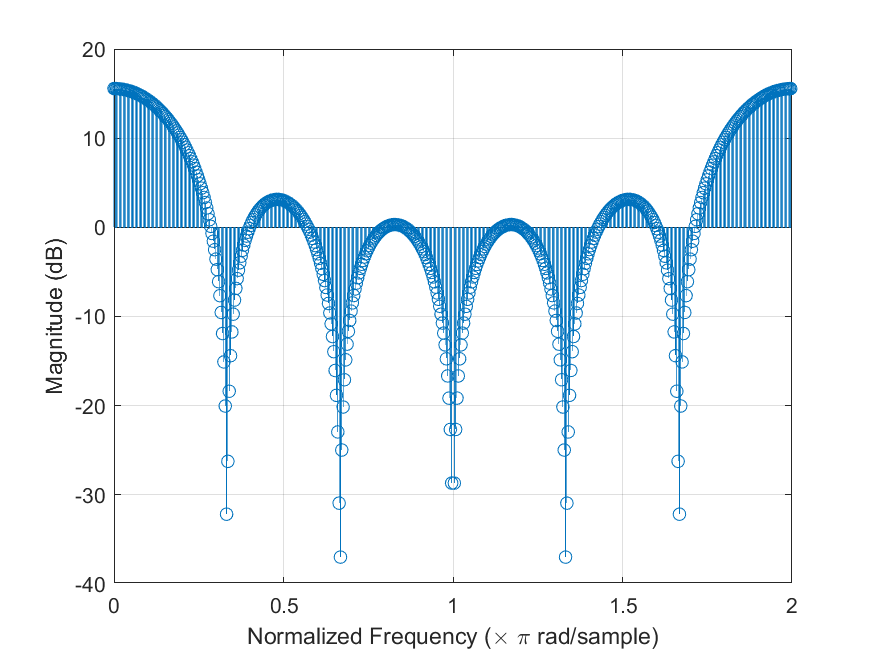
\includegraphics[width=0.5\columnwidth]{assignment_01/plots/5th_order_running_sum_freq_resp.png}
        \label{fig:freq_resp1_b}
    }
    \caption{Frequency response of two running sum filters plotted on the normalized-frequency axis.}
    \label{fig:freq_resp1}
\end{figure}
\begin{comment}
\begin{figure}[h]
    \centering
    \captionsetup[subfloat]{farskip=0pt,captionskip=0pt}
    \subfloat[\nth{3} order moving average]{
        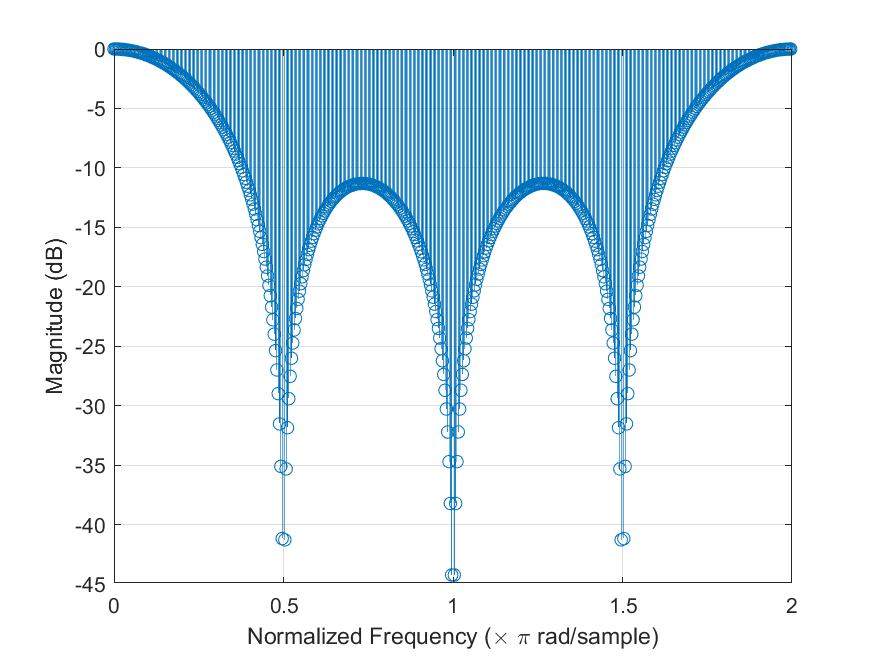
\includegraphics[width=0.5\columnwidth]{assignment_01/plots/3rd_order_moving_average_freq_resp.png}
        \label{fig:freq_resp2_a}
    }
    \subfloat[\nth{5} order moving average]{
        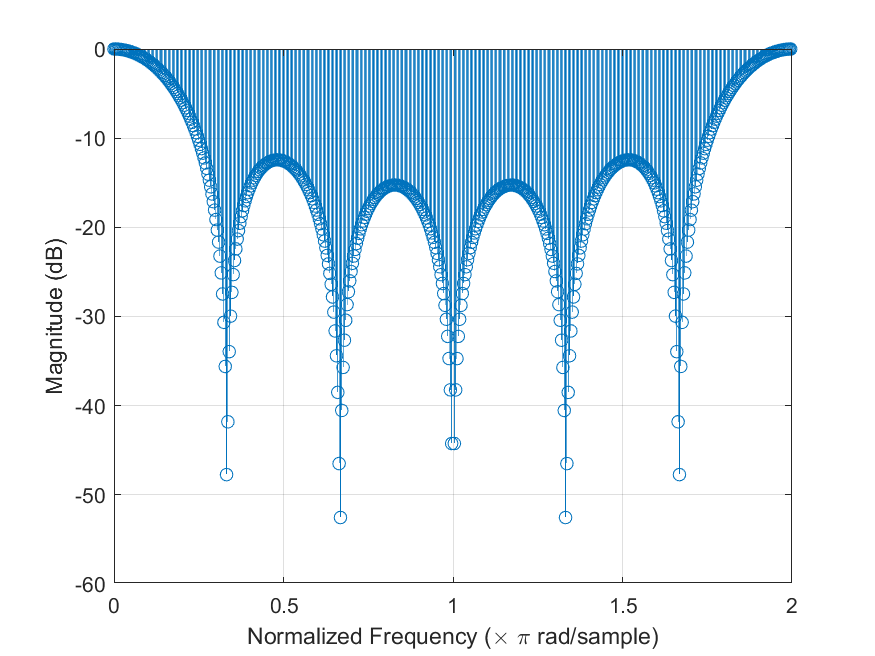
\includegraphics[width=0.5\columnwidth]{assignment_01/plots/5th_order_moving_average_freq_resp.png}
        \label{fig:freq_resp2_b}
    }
    \caption{Frequency response of two moving average filters plotted on the normalized-frequency axis.}
    \label{fig:freq_resp2}
\end{figure}
\end{comment}

\newpage

\section{Room model using sound reflections}

In this section two system models for the acoustic behavior of a room are examined. Both models try to capture the reflection of sound waves of the rooms walls. The first model achieves this using a single reflection after a certain delay, resulting in a FIR filter. The other model uses feedback to create a never ending series of increasingly attenuated reflections, resulting in an IIR filter.

The FIR filter is described by the difference equation:
\begin{equation}
    y(n) = x(n) + \alpha x(n-delay)
\end{equation}

This can be transformed to the z-domain resulting in:
 \begin{equation}
     Y(z) = X(z) + \alpha X(z) z^{-delay}
 \end{equation}
 \begin{equation}
     H_{FIR}(z) = \frac{z^{delay} + \alpha}{z^{delay}}
\end{equation}

The IIR filter on the other hand is described by the difference equation:
\begin{equation}
    y(n) + \alpha y(n-delay) = x(n)
\end{equation}

The z-domain transfer function can be determined to be:
\begin{equation}
    Y(z) + \alpha Y(z) z^{-delay} = X(z)
\end{equation}
\begin{equation}
    H_{IIR}(z) = \frac{z^{delay}}{z^{delay} + \alpha}
\end{equation}

We can see that the transfer functions of the two models are actually the inverse of each other. The FIR filter has $delay$ zeros spread evenly around the unit circle and a pole at the origin with a multiplicity of $delay$ and vice versa for the IIR model.

The inverse nature of the two models also becomes apparent in their spectra. Figure \ref{fig:bounce:spectra} shows a small section of the very densely packed spectra of two FIR and IIR implementations using a time delay of $\SI{10}{ms}$ and $\SI{200}{ms}$ resulting,  at a sampling frequency of $\SI{44.1}{kHz}$, in delays of 441 and 8820 samples, respectively. Both use a value of 0.6 for $\alpha$. It can be observed that the spectra are periodic and that the period is determined by the time delay of the implementation.

When studying the impulse responses (see figure \ref{fig:bounce:impulse}) the similarities between the two models vanish but we can see the expected behavior: The FIR filter repeats the input signal slightly attenuated once after a certain number of samples whereas the IIR reflects an increasingly attenuated version of the input signal indefinitely.

The effect of the two filter models on a signal can be studied in figure \ref{fig:bounce:signals}. The reflected versions of the signal add to the original signal and make it harder to identify. This translates to the original signal being harder to hear when listening to the filtered version. The longer the time delay, the larger the number of different reflections that add to the original signal in a small time interval and the original signal gets even less identifiable. Since the IIR filter produces a never ending series of reflection, it creates signals where the original signal is hardest to identify.

Listening to both filters, the IIR based filter clearly sounds more realistic and thus seems to be the superior model.

\begin{figure}
    \centering
    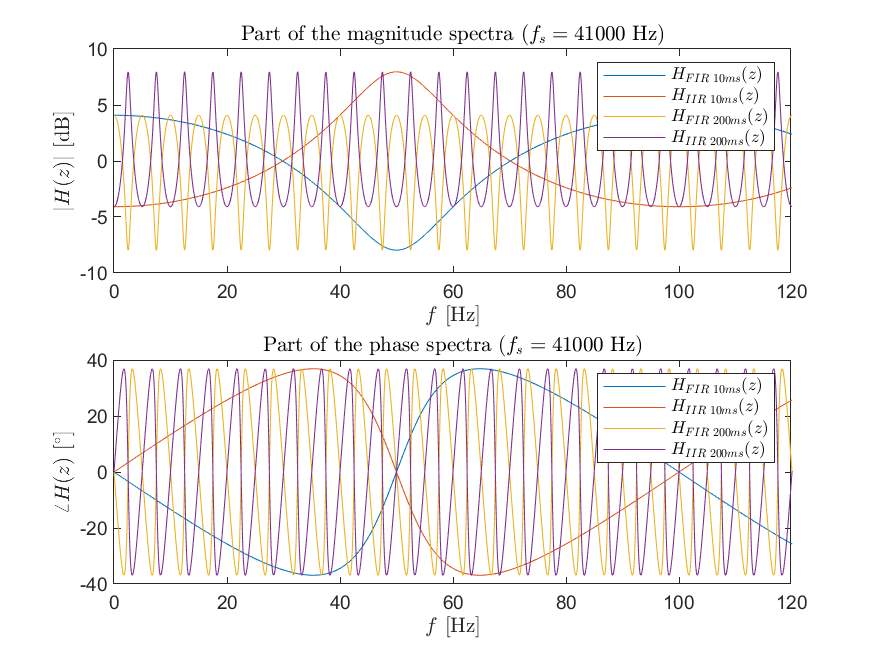
\includegraphics[width=\linewidth]{assignment_01/plots/bounce_spectra.png}
    \caption{Part of the spectra for both room models with two different time delays.}
    \label{fig:bounce:spectra}
\end{figure}
\begin{figure}
    \centering
    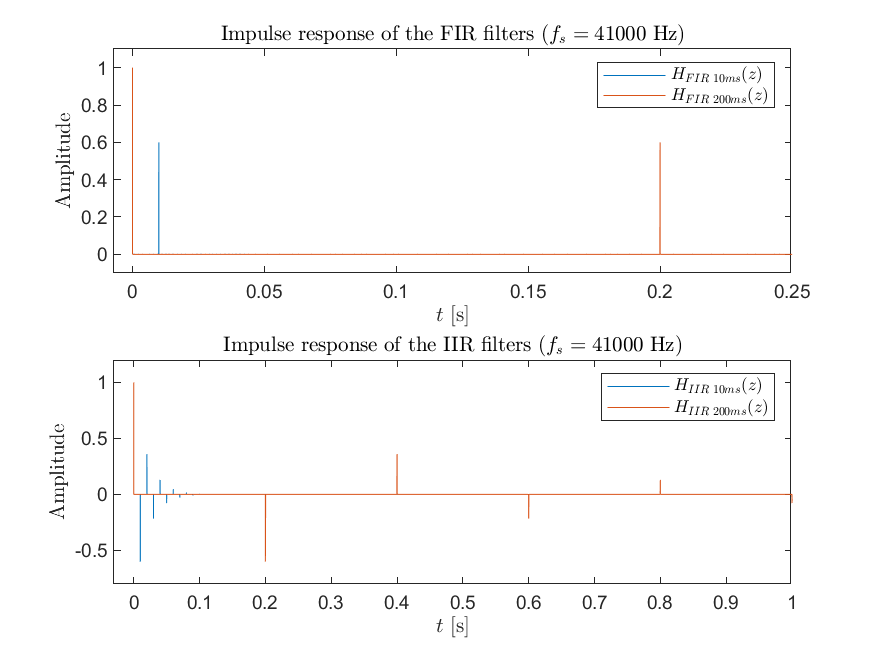
\includegraphics[width=\linewidth]{assignment_01/plots/bonuce_impulse.png}
    \caption{Impulse responses for both room models with two different time delays.}
    \label{fig:bounce:impulse}
\end{figure}
\begin{figure}
    \centering
    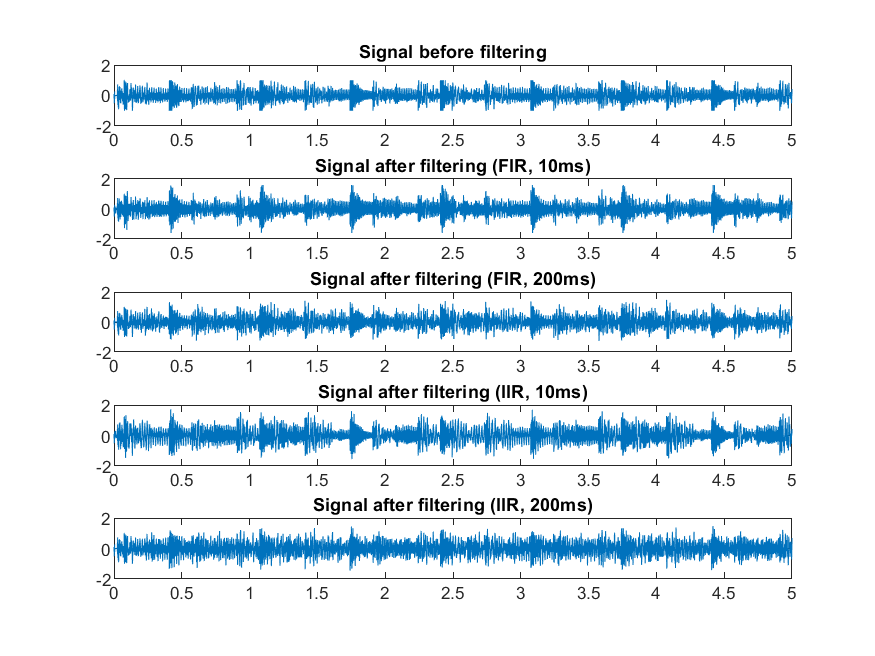
\includegraphics[width=\linewidth]{assignment_01/plots/bounce_signals.png}
    \caption{Application of the two models on a signal for two different time delays.}
    \label{fig:bounce:signals}
\end{figure}

\clearpage
\newpage

\section{Results}
Describe the results you obtained. Make sure you mention all the correct points and refer to the figures you produced.

\section{Discussion}
Provide some more general comments putting the specific points you found out in the single parts into a bigger context and how they connect to the rest of the conbtants of the course.



\clearpage
\section{Fourier transform of a recorded signal (Hands-on 3)}
% first have a section with a short explanation of fourier transform mathematically, then go into the details of the exercise and what the following sections describe/show/include and also the results 
To analyze the composition of a recorded signal, it is often more practical to examine it in the frequency domain. To move from the time-domain into the frequency domain, we use Fourier transform. 
\newline
\textit{\textbf{Show equations for discrete fourier and inverse fourier?}}
\newline
Hands-on 3 exercise 1.3 dealt with the Fourier transform of a recorded signal. The sound sample of a piano playing a single note 'piano.wav' was loaded into MATLAB. The discrete time signal 'piano.wav' is made up of many frequency components, and the Fourier transformation is a sort of decomposition of the signal into its frequencies. As a result, we can see how much of each frequency is contained within the signal.


\subsection{Signal plots and Fourier transform}
% describe the methods used, and explain why you choose your specific approach! restrict yourself to the most essential information. provide all information necessary to reproduce your results
In order to learn about the composition of the sound signal, the signal was plotted in the time and frequency domain (see figure \ref{fig:time} and \ref{fig:freq}). 

\begin{figure} [h]
    \centering
    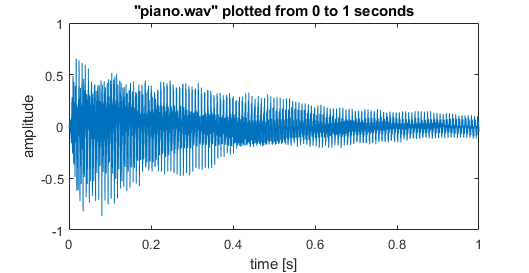
\includegraphics[width=\linewidth]{assignment_01/plots/time_plot.png}
    \caption{Recorded signal plotted in the time-domain from 0 to 1 s.}
    \label{fig:time}
\end{figure}
\begin{figure} [h]
    \centering
    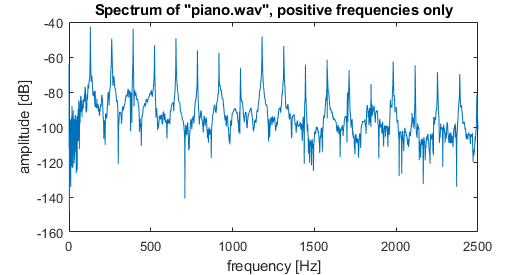
\includegraphics[width=\linewidth]{assignment_01/plots/freq_plot.png}
    \caption{Power spectrum of recorded signal. Only positive frequencies, including the DC component, are shown; specifically 0 to 2500 Hz.}
    \label{fig:freq}
\end{figure}

We use discrete Fourier transform to get the spectrum of the whole signal in MATLAB. It is important to note, that MATLABs fft function returns the positive values of the signal spectrum first. The spectrum of the whole signal is plotted with \textit{Hz} and \textit{dB} on the x- and y-axis respectively. % should we show this plot?
To plot only the positive frequencies, including the DC component, we create new frequency and signal vectors, only containing values for the positive frequencies. The resulting plot is shown in figure \ref{fig:freq}.

\textbf{\textit{(Describe how the frequency vector is made (intervals, start and end-points)?)}}

\newline
From the spectrum in figure \ref{fig:freq}, we can estimate the fundamental frequency of the signal by looking at the spectral peaks. The fundamental frequency is defined as the lowest frequency of a periodic waveform. % wikipedia
We see that the lowest peak is found at 130.43 Hz and therefore, with a precision of 0.5 Hz, we estimate the fundamental frequency of the signal to be
\begin{equation}
    f_0 = 130.5 Hz.
\end{equation}

The fundamental frequency is what we perceive as the musical pitch of a tone. 130.5 Hz roughly correlates with the fundamental of C3 on a piano, which sounds very similar to the tone played in 'piano.wav'. The other peaks in the spectrum represent the harmonics of the tone. 

\subsection{Synthesis and inverse Fourier transform}
Using the distribution of harmonics from the power spectrum, we can synthesize the sound of a piano. 
% "we synthesize the signal with a length of 2 s in the frequency domain by approximating it via a harmonic series: ..."
\textbf{\textit{explain synthesis and why we use inverse Fourier and what is does...}}
\newline
\textit{Plot...}
\newline
For the synthesized signal to sound like a realistic piano, the harmonics of the signal have to have the right distribution and amplitude in relation to each other. Otherwise, the result might as well sound like another instrument. 


% compare the synthesized signal, how does it compare - especially in the power spectrum - if the harmonics are different/have different magnitudes, we would expect the human ear to notice a difference - wouldnt sound like piano without power in the higher harmonics
% see rubrics on learn

% "magnitude spectrum"
% should the spectra be plottes with sticks instead of "continously"?
% our signal has finite duration 
% spectral resolution is dependent on signal length in time

\end{document}


